\documentclass{article}
\usepackage{ctex}
\usepackage[top=2.5cm,left=2cm,right=2cm,bottom=2cm]{geometry}
\title{社区居民问卷小样}
\author{}
\date{}
\usepackage{setspace}
\usepackage{fancyhdr}
\usepackage{graphicx}
\graphicspath{{images/}}
\usepackage{subfigure}
\pagestyle{empty}
\begin{document}
\maketitle
\clearpage
\begin{spacing}{1.0}
您好,这是一份由南京中医药大学第一临床医学院发起的调查问卷,旨在了解社区居民对于社区卫生服务中心服务的参与情况以及对于中医预防保健工作开展的意见。该问卷依托于“中医治未病理论的社区知信行调查”。

本问卷时长约五分钟,我们郑重承诺,本问卷的所有数据仅用于科研用途,您的所有个人信息将受到相关法律的保护。


\begin{enumerate}
\item 过去的一年您去过几次社区卫生服务中心?

A.0次 \qquad
B.1-2次\qquad
C.2-5次\qquad
D.5次以上

\item 您是因为什么原因去的?(可多选)

A.治疗疾病 \qquad
B.预防保健\qquad
C.职工体检\qquad
D.其他(填写)\underline{\makebox[6em]{}}

\item 您治疗的哪一类疾病?(可多选)

A.上呼吸道感染,如感冒、咳嗽\qquad
B.胃肠疾病\qquad
C.慢性疾病\qquad
D.其他(填写)\underline{\makebox[6em]{}}

\item 您选择了中医治疗还是西医治疗?

A.中医\qquad
B.西医(转至第六题)\qquad
C.都有

\item
您接受了哪一种中医治疗?(可多选)

A.草药煎汤\qquad B.贴敷的膏药\qquad 
C.物理疗法,比如针灸,拔火罐等\qquad D.其他(填写)\underline{\makebox[6em]{}}

\item 您接受了哪一种保健项目?(可多选)

A.草药调理\qquad
B.针灸、推拿\qquad
C.中医体质辨识\qquad
D.贴敷膏药\qquad
E.膏方

\item 您有听说过“治未病”这一概念吗?

A.有\qquad
B.没有\qquad
C.不清楚

\item 您认为“治未病”一词的含义是指什么?(可多选)

A.预防未发生的疾病\qquad B.生病后防止病情进展\qquad C.病后预防疾病再次复发

\item 您了解中医养生知识的途径是以下哪些?(可多选)

A.社区宣传\qquad B.亲戚朋友推荐\qquad C.医生\qquad
D.电视\qquad
E.互联网\qquad
F.其他途径(填写)\underline{\makebox[6em]{}}

\item 
您的
性别\underline{\makebox[6em]{}}
年龄\underline{\makebox[6em]{}}
学历\underline{\makebox[6em]{}}
年收入情况\underline{\makebox[6em]{}}

感谢您的参与以及对我们的支持!
\end{enumerate}
\begin{figure*}
    \begin{minipage}{3cm}
    \flushleft

\includegraphics[width=3cm]{qrcode.jpg}
    \end{minipage}
\begin{minipage}{2cm}
 \flushleft
    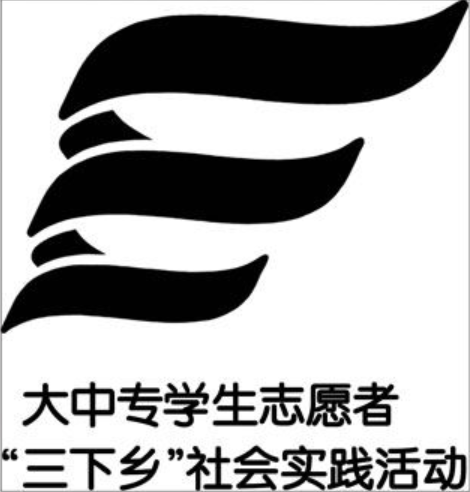
\includegraphics[width=2cm]{xiaxiang.png}
\end{minipage}
\end{figure*}
\end{spacing}

\end{document}